\mysubsubsection{Lurking Behaviors and Initial Contact}
We explored lurking behavior of our students, and found that projects present in Github and those projects having a FAQ had longer lurking times, where as projects having formal on boarding material had or beginner bugs identified made lurking time lower (see Table \ref{tab:lurking_time_regression}). This model has rather good fitness (adj. $r^2$ 0.134); however other than the Github factor fail to achieve statistical significance\footnote{Without the beginner bug question, we can report significantly higher adj. $r^2$ in 0.185 without effects on other questions significance}.

\begin{table}
\begin{tabular}{lrrr}
Factor & $\beta$ & stand. $\beta$ & sig \\
\hline 
Uses Github & 2.291\newline1.170 & 0.480 & 0.071 * \\ 
Has newcommer bugs & -0.309\newline0.906 & -0.081 & 0.739 \\ 
Has a FAQ & 1.114\newline0.834 & 0.290 & 0.203 \\ 
Has onboarding instructions & -1.372\newline0.975 & -0.352 & 0.181 \\
\hline
Participant has previous OS experience & 0.104\newline0.737 & 0.032 & 0.890 \\ 
\hline 
\end{tabular} 
\caption{Explaining lurking time}
\label{tab:lurking_time_regression}
\end{table}

These results draw a mixed figure of the phenomena; having a FAQ might indicate complexity of the project or the level of institutionalization, which could explain our finding. However, the negative factor on on-boarding instruction indicates that lurking might not be only about getting familiar with the community, rather also following and understanding the behaviors of the community, often explicated in on-boarding information. 

We found it interesting that open source development was clearly a non-significant factor and that the coefficient is approximately zero, therefore indicating that this control variable has no impact on this.


Most of the participants answered that they {\bf have been lurking} prior to contacting the project, although the days of lurking are widely spread among the projects. {\it 21\%} answered that the question is not applicable for them and their project. 


\begin{figure}[ht!]
\centering
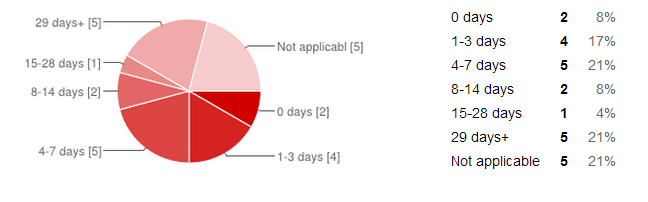
\includegraphics[width=90mm]{chapters/img/lurking_response.png}
\caption{Lurking Response}
\label{overflow}
\end{figure}

Coming to intial contact, about half of the people used mail to get into contact with the community (either through a private mail or to the mailing list). Social media was only used by one participant \footnote{Fogel pointed out that social networks might have an impact on OS, but the impact is still not well understood.}. This suggests that mail is still the main form of communication, at least for initial communication.


\begin{figure}[ht!]
\centering
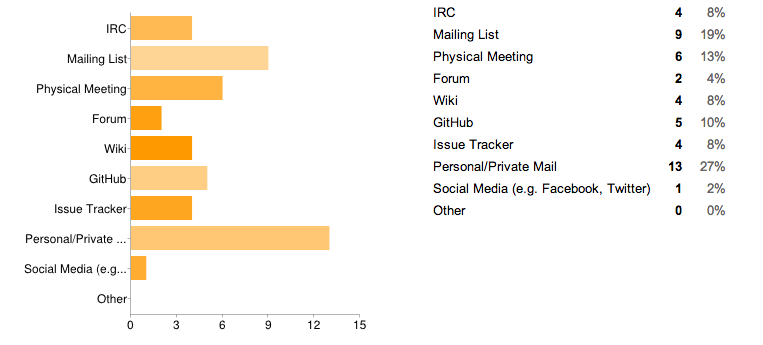
\includegraphics[width=120mm]{chapters/img/initial_contact.png}
\caption{Initial Contact }
\label{overflow}
\end{figure}